\label{sec:hadhad_multijet}

Multi-jet production is a source of background in the \hadhad signal
region where both \tauhadvis candidates originate from the
misidentification of quark- or gluon-initiated jets. It represents the
second largest background with \faketauhadvis in the \hadhad SR after
the dominant \ttbarFakes contribution.

\subsubsection{The fake factor method}

The multi-jet background is estimated using the fake factor method
which is a data-driven method for background estimation. It is
applicable in cases where two event observables exist that are
statistically independent for the background process to be estimated,
while also being strong discriminators between the background and
other processes (signal and non-multi-jet processes). Four disjoint
regions can be defined, three background-enriched control regions and
a signal-like region, by performing a binary categorisation for each
observable. The assumption of statistical independence allows to
relate the expected number of events for the background process
between the control regions and the signal-like region, thus yielding
a data-driven estimate of the expected background contribution in the
signal-like region.

In the \hadhad channel, two observables allowing to define control
regions enriched in multi-jet events are the \tauid requirements
applied to \tauhadvis candidates and the sign of the electric charges
of both candidates.

In the signal region, \tauhadvis candidates are required to pass the
loose \tauid working point. This requirement defines regions where
both \tauhadvis candidates pass \tauid which are herafter referred to
as ID regions. The selection is partially inverted to obtain control
regions enhanced in multi-jet events by requiring that exactly one
\tauhadvis candidate is failing the loose \tauid working point, while
still passing a working point corresponding to an efficiency loss of
\tauhad of about 1\,\% ($\text{RNN score} > 0.01$). The \tauhadvis
candidates fulfilling this selection are referred to as
anti-\tauhadvis and the regions defined by the inversion of the
identification criterion as Anti-ID regions. The identification
criterion cannot be fully inverted due to
pre-selections\footnote{Datasets targeting $\PHiggs \to \hadhad$
  require events with at least one \tauhadvis passing the loose \tauid
  working point and one \tauhadvis with an RNN \tauid score exceeding
  0.01.} applied in the data reduction pipeline of the ATLAS
experiment. However, the fake factor method is still valid in the
presence of these constraints.

The electric charge of both \tauhadvis candidates produced from signal
processes and dominant sources of backgrounds with two \tauhadvis
orginating for hadronic $\tau$~decays ($\PZ \to \tautau$,
$\PHiggs \to \tautau$, \ttbar) are expected to be reconstructed with
opposite-sign (OS) electric charge. The OS requirement is inverted
yielding regions with \tauhadvis candidates of same-sign (SS) electric
charge, depleting the region of processes where both \tauhadvis
orginate from hadronic $\tau$ decays. In contrast, the multi-jet
background contributes similarly to the OS and SS regions since
\tauhadvis charge reconstruction has little sensitivity to the
relative sign of the electric charge between partons initiating jets
that are being misidentified as \tauhadvis.

With the previously defined control regions and assumption of
independence of both categorical observables, the expected multi-jet
contribution in regions with \tauhadvis passing loose identification
and with \tauhadvis pairs of opposite-sign electric charge can be
estimated using
\begin{align*}
  N_\text{multi-jet}^{\text{OS, ID}} =
  N_\text{multi-jet}^{\text{OS, Anti-ID}}
  \cdot
  \underbrace{\frac{N_\text{multi-jet}^{\text{SS, ID}}}
  {N_\text{multi-jet}^{\text{SS, Anti-ID}}}}
  _{= \text{FF}_\text{SS}} \,\text{,}
\end{align*}
where $N_\text{multi-jet}$ is the number of multi-jet events in a
given region. The fake factor (FF) measures the ratio of multi-jet
events in the ID and Anti-ID region\footnote{The use of identification
  or isolation criteria to define the ratio is the main difference
  between the fake factor method and the more general ABCD method.}.

The probability of misidentifying a quark- or gluon-jet as a hadronic
$\tau$ decay depends strongly on the properties of the reconstructed
\tauhadvis candidate. Particularly, the reconstructed decay mode and
visible transverse momentum affect the probability of a jet
reconstructed as a \tauhadvis to pass \tauid (cf.\
\Cref{sec:tauid}). To control for this effect, fake factor
measurements are frequently performed in bins of observables related
to properties of reconstructed \tauhadvis.

The control regions defined by inverting the OS and ID requirements on
\tauhadvis do not provide pure samples of multi-jet events. Therefore,
number of multi-jet events is estimated according to
\begin{align*}
  N_\text{multi-jet} = N_\text{data} - N_\text{non-multi-jet} \,\text{,}
\end{align*}
where $N_\text{data}$ is the observed number of events in the
multi-jet enriched region and $N_\text{non-multi-jet}$ the expected
contribution of non-multi-jet events estimated using simulation.

In~\Cref{tab:mjfakes_yields} the multi-jet and non-multi-jet yields in
the regions relevant for the \faketauhadvis estimation are
summarised. The 2 $b$-tag region, while most similar to the signal
region, is not well suited to estimate fake factors:
\begin{itemize}

\item The 2 $b$-tag regions used in the fake factor method have a
  large contamination from non-multi-jet backgrounds, primarily
  \ttbarFakes, that have to be subtracted. The large size of the
  subtraction leads to a degradation of the statistical precision of
  measured fake factors and introduce large systematic uncertainties
  originating from the modelling of the subtracted components.

\item The \btag requirement suppresses the multi-jet contribution in
  the control regions preventing a differential measurement of fake
  factors in properties of the \tauhadvis.

\item The multi-jet estimate cannot be validated in the 2 $b$-tag
  region due to the absence of a region with high multi-jet purity
  that is similar to the signal region.

  % Resultingly, the statistical independence of the charge sign and ID
  % observables employed by the FF method cannot be verified.
\end{itemize}
These issues are addressed by performing the fake factor measurement
in the 1 $b$-tag region, which has a higher abundance and purity of
multi-jet events, and extrapolating the measurement into the 2 $b$-tag
region to obtain a multi-jet background estimate in the signal region.

\begin{table}[htbp]
  \centering

  \begin{subtable}[t]{\textwidth}
    \centering
    % Size of subtraction and multi-jet purity:
%                         multi_jet  non_multi_jet  multi_jet_error  non_multi_jet_error  multi_jet_purity
% anti_id charge_sign
% False   OS           16067.048497   16443.951503       204.558258            96.607872          0.494203
%         SS           14040.394005    1971.605995       129.147367            25.827164          0.876867
% True    OS           91582.182374   13677.817626       334.090987            79.729466          0.870057
%         SS           78399.983641    5707.016359       296.470480            61.544664          0.932146

\begin{tabular}{
  ll
  S[table-format=5.0(3)]
  S[table-format=5.0(3)]
  c}
  \toprule
  \multicolumn{2}{l}{Region} & {$N_\text{multi-jet}$} & {$N_\text{non-multi-jet}$} & {Multi-jet purity} \\
  \midrule
  \multirow{2}{*}{SS} & ID      & 14040 +- 130 & 1970 +- 30   & 88\,\% \\
                      & Anti-ID & 78400 +- 300 & 5710 +- 70   & 93\,\% \\
  \midrule
  \multirow{2}{*}{OS} & ID      & 16070 +- 210 & 16440 +- 100 & 49\,\% \\
                      & Anti-ID & 91580 +- 340 & 13680 +- 80  & 87\,\% \\
  \bottomrule
\end{tabular}



%%% Local Variables:
%%% mode: latex
%%% TeX-master: "../phd_thesis"
%%% End:

    \subcaption{1 $b$-tag regions}
    \label{tab:mjfakes_yields_1tag}
  \end{subtable}

  \begin{subtable}[t]{\textwidth}
    \centering
    % Size of subtraction and multi-jet purity:
%                        multi_jet  non_multi_jet  multi_jet_error  non_multi_jet_error  multi_jet_purity
% anti_id charge_sign
% False   OS            408.197943    7971.802057       105.950917            53.344135          0.048711
%         SS           1299.622259    1001.377741        50.345854            15.287412          0.564808
% True    OS           8429.603396    8864.396604       139.699303            47.136984          0.487429
%         SS           7653.735896    3338.264104       108.557939            28.157166          0.696301

\begin{tabular}{
  ll
  S[table-format=5.0(3)]
  S[table-format=5.0(3)]
  c}
  \toprule
  \multicolumn{2}{l}{Region} & {$N_\text{multi-jet}$} & {$N_\text{non-multi-jet}$} & {Multi-jet purity} \\
  \midrule
  \multirow{2}{*}{SS} & ID      & 1300 +- 60  & 1000 +- 20 & 56\,\% \\
                             & Anti-ID & 7650 +- 110 & 3340 +- 30 & 70\,\% \\
  \midrule
  \multirow{2}{*}{OS} & ID      & \multicolumn{3}{c}{\rule[3pt]{5.2em}{0.3pt}\hspace{1em}Signal Region\hspace{1em}\rule[3pt]{5.2em}{0.3pt}} \\
                             & Anti-ID & 8430 +- 140 & 8860 +- 50 & 49\,\% \\
  \bottomrule
\end{tabular}




%%% Local Variables:
%%% mode: latex
%%% TeX-master: "../phd_thesis"
%%% End:

    \subcaption{2 $b$-tag regions}
  \end{subtable}

  \caption{Number of multi-jet events in regions defined by different
    \tauhadvis pair electric charge (OS, SS) and \tauhadvis
    identification (ID, Anti-ID). The number of multi-jet events,
    $N_\text{multi-jet}$, is estimated by subtracting the number
    non-multi-jet events, $N_\text{non-multi-jet}$, estimated using
    Monte Carlo simulation from the observed number of events in this
    region. In (a) the breakdown is shown after a 1 $b$-tag
    requirement; in (b) after a 2 $b$-tag requirement (the SR -- 2
    $b$-tag OS ID -- is omitted). The uncertainties are from
    statistical sources only.}
  \label{tab:mjfakes_yields}
\end{table}

A schematic illustration of this approach is given
in~\Cref{fig:fakefactor_regions}. Fake factors measured in the 1
$b$-tag regions ($\text{FF}_\text{SS}^\text{1-tag}$) are applied to
events in the 2 $b$-tag OS Anti-ID region after subtraction of
non-multi-jet contributions to obtain multi-jet templates in the
signal region. Multiplicative transfer factors
($\text{TF}_{1 \ra 2\,b\text{-tag}}$) are applied to
$\text{FF}_\text{SS}^\text{1-tag}$ when used in 2 $b$-tag regions,
absorbing possible differences between fake factors measured in 1 and
2 $b$-tag regions and the uncertainties associated with this
extrapolation.

\begin{figure}[htbp]
  \centering

  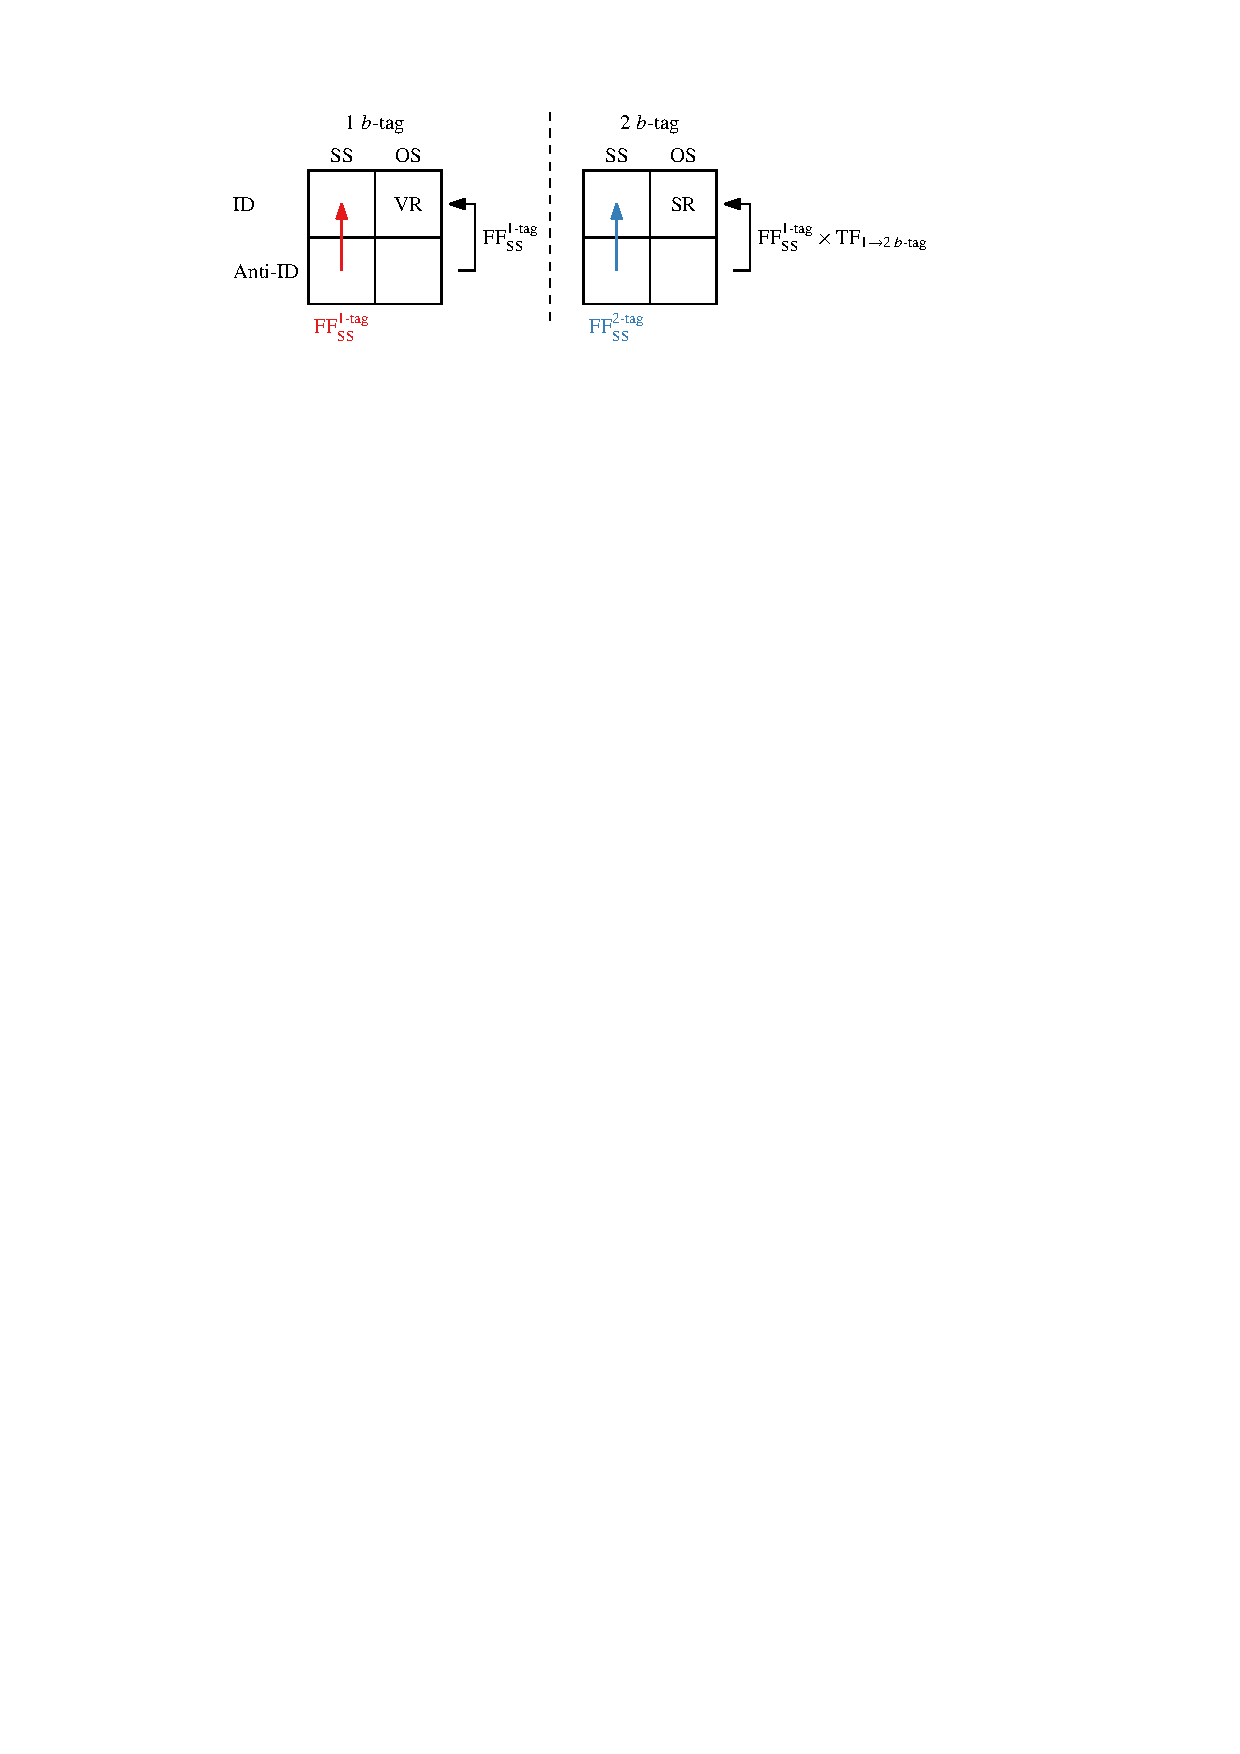
\includegraphics[scale=1]{fakefactors/regions}

  \caption{Schematic description of the fake factor method employed to
    estimate the multi-jet background in the signal region of the
    \hadhad channel. The squares represent the multi-jet events
    ($N_\text{multi-jet} = N_\text{data} - N_\text{non-multi-jet}$) in
    a particular region.}
  \label{fig:fakefactor_regions}
\end{figure}

The 1 $b$-tag OS ID region serves as a validation region to check the
closure of the multi-jet estimate and thus verify the independence of
the categorical observables related to \tauid (ID / Anti-ID) and
electric charge of the \tauhadvis pair (OS / SS). This approach is
equivalent\todo{Is it really? I don't think so.} to a comparison of
fake factors measured in the OS and SS
regions\footnote{\Cref{tab:mjfakes_yields_1tag} can be used to
  calculate inclusive fake factors in the OS and SS regions, yielding
  $\text{FF}_\text{SS}^\text{1-tag} \approx
  \text{FF}_\text{OS}^\text{1-tag} \approx 0.18$, which is a
  sufficient condition for statistical independence of the fake factor
  observables at the level of the inclusive selection.}, which have to
agree under the assumptions of the method.


\subsubsection{Measurement of fake factors}

% - STT / DTT binning
The fake factor measurement is performed separately for events
selected by single- and di-\tauhadvis triggers as well as the years of
data collection. During Run~2 of the LHC, different \tauhadvis trigger
chains were used by the ATLAS experiment to collect the data used in
this analysis. As a result, the topologies of the selected events and
the \tauid applied at the high-level trigger changed as Run~2
progressed. To account for possible differences resulting from the
change in trigger-selection, the fake factor measurement is subdivided
into three major data collection periods: 2015-2016, 2017, and
2018. The 1 $b$-tag regions relevant to the measurement of fake
factors are shown in~\Cref{fig:mjfakes_1tag_ss_plots}.

\begin{figure}[htbp]
  \centering

  \begin{subfigure}{0.49\textwidth}
    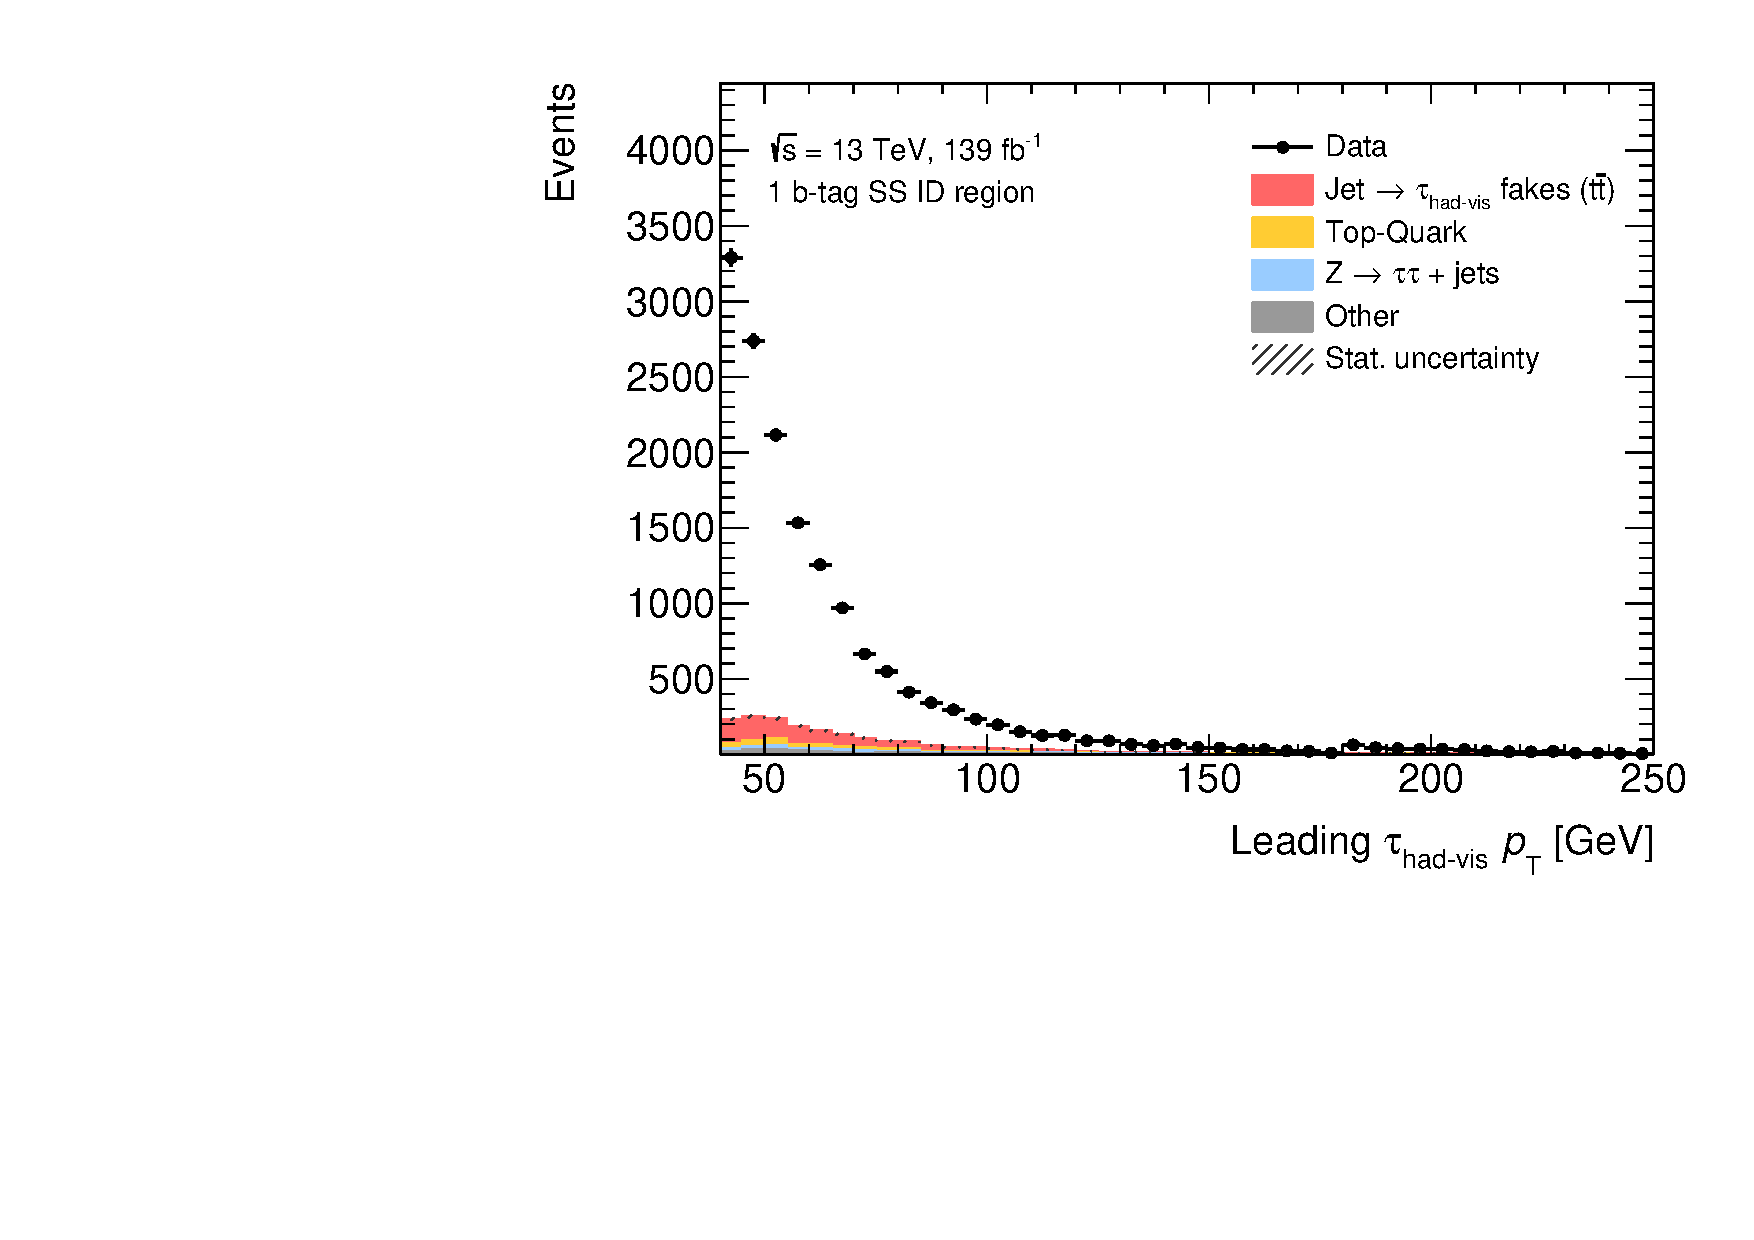
\includegraphics[width=\textwidth]{fakefactors/region_plots/tau0pt_1tag_ss_id}
    \subcaption{Leading \tauhadvis \pT in the 1 $b$-tag SS ID region}
  \end{subfigure}
  \begin{subfigure}{0.49\textwidth}
    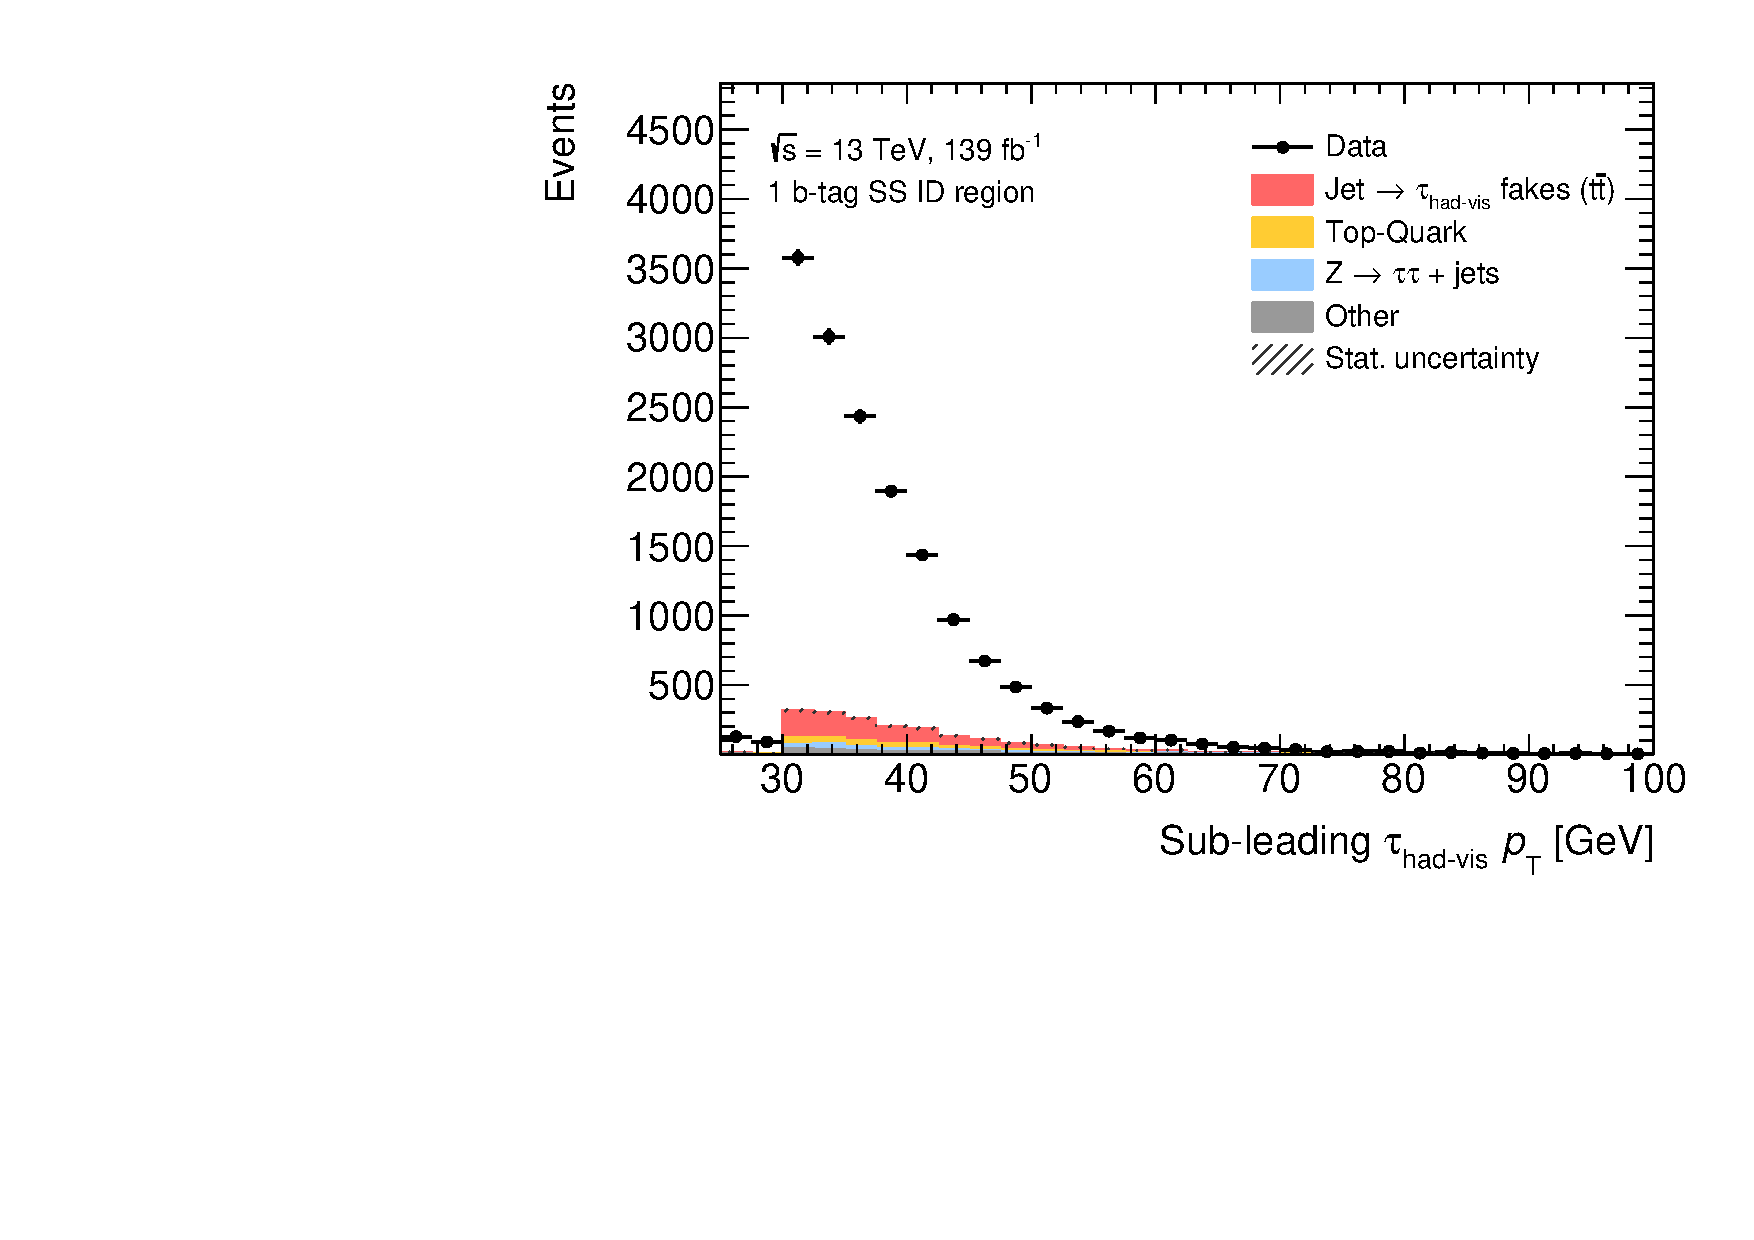
\includegraphics[width=\textwidth]{fakefactors/region_plots/tau1pt_1tag_ss_id}
    \subcaption{Sub-leading \tauhadvis \pT in the 1 $b$-tag SS ID
      region}
  \end{subfigure}

  \begin{subfigure}{0.49\textwidth}
    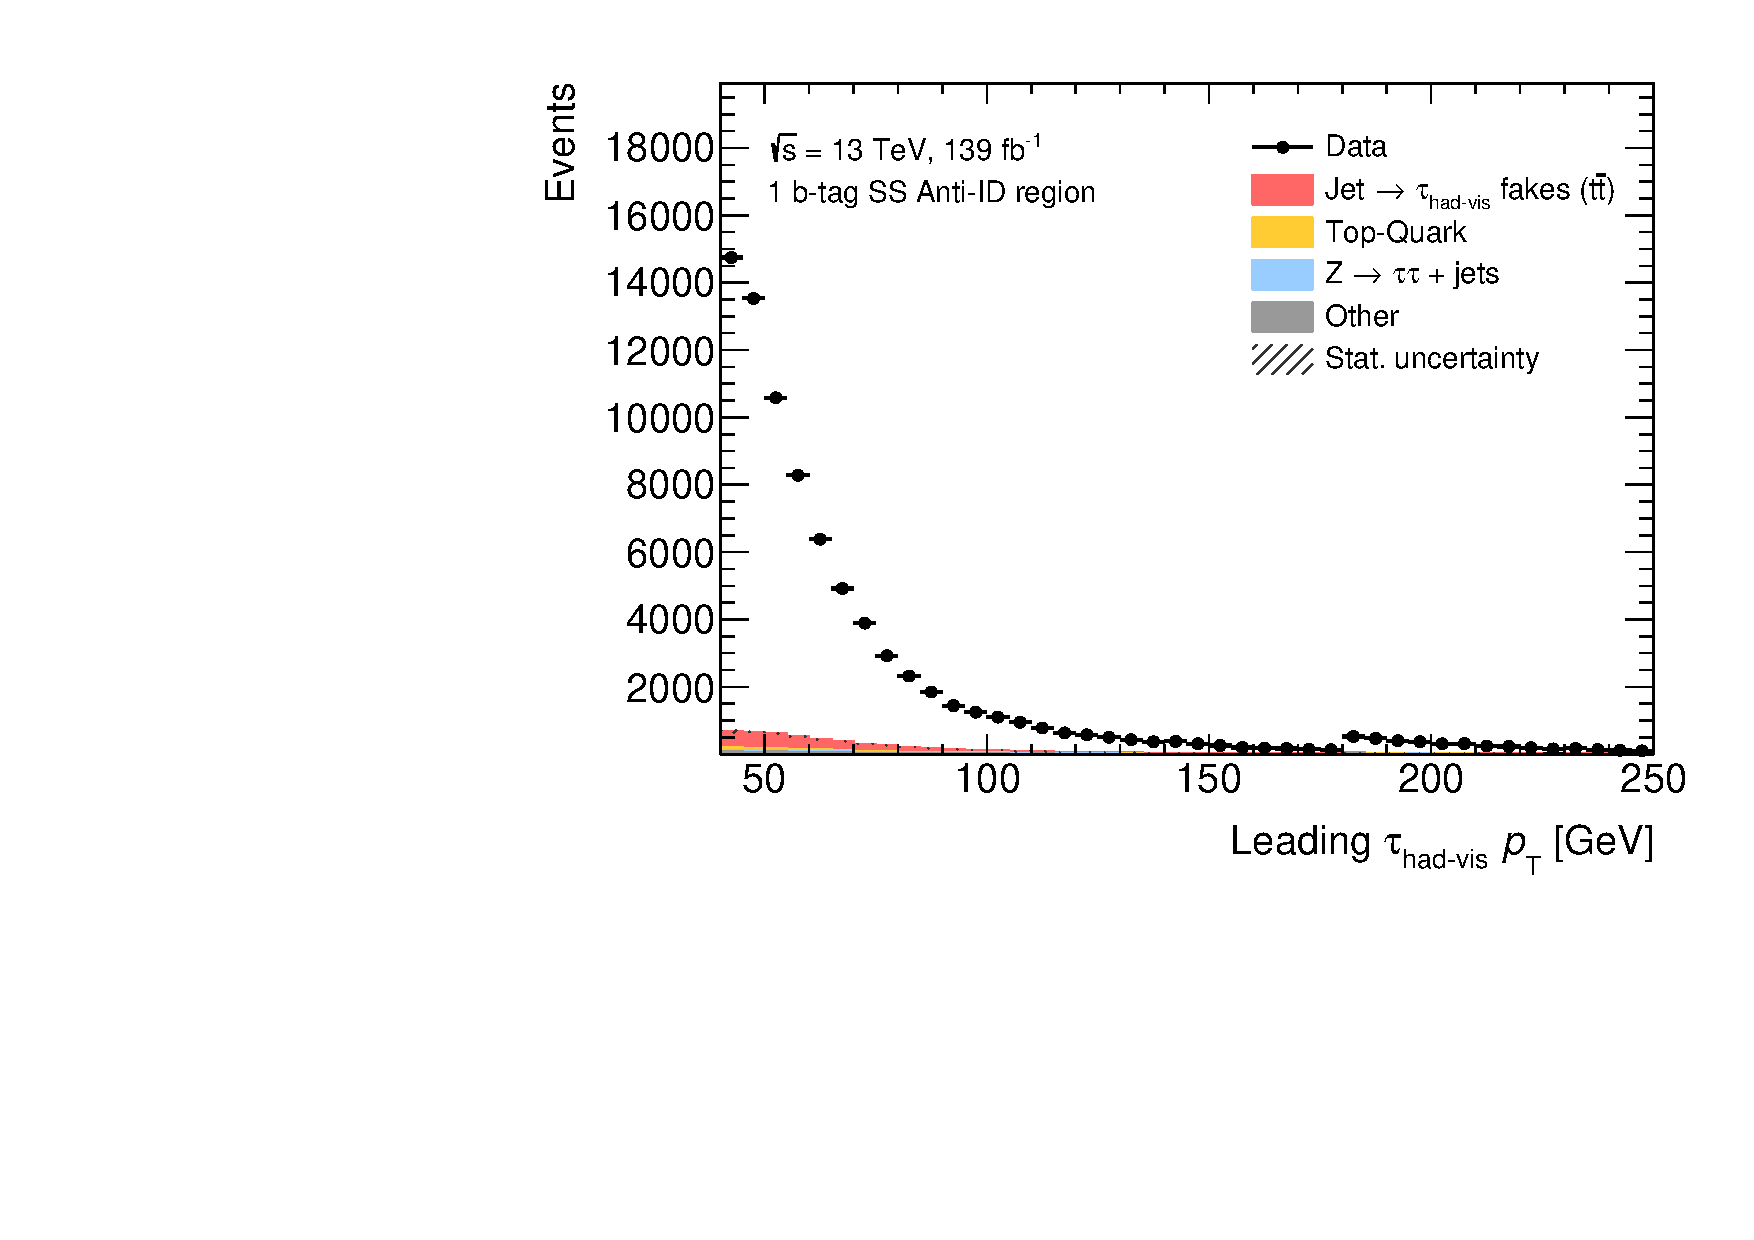
\includegraphics[width=\textwidth]{fakefactors/region_plots/tau0pt_1tag_ss_antiid}
    \subcaption{Leading \tauhadvis \pT in the 1 $b$-tag SS Anti-ID region}
  \end{subfigure}
  \begin{subfigure}{0.49\textwidth}
    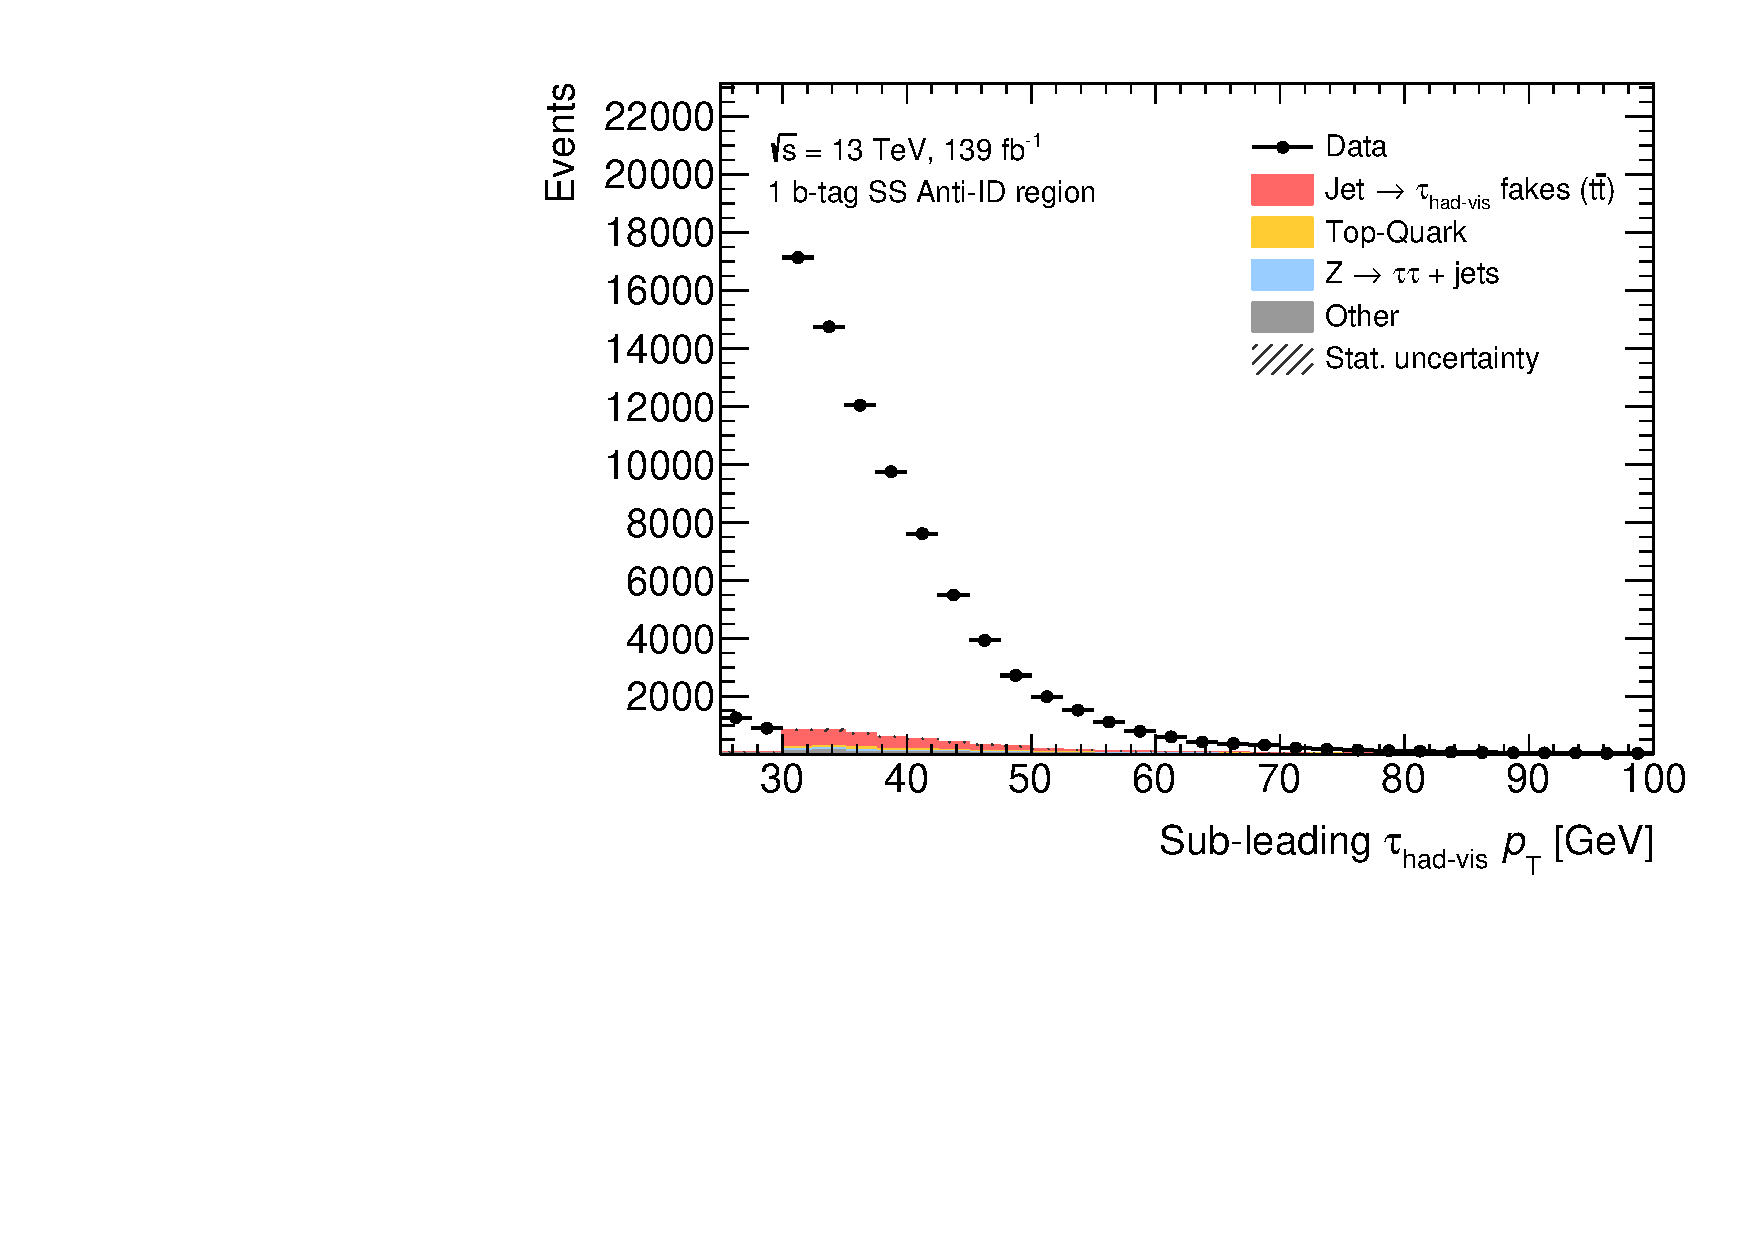
\includegraphics[width=\textwidth]{fakefactors/region_plots/tau1pt_1tag_ss_antiid}
    \subcaption{Sub-leading \tauhadvis \pT in the 1 $b$-tag SS Anti-ID
      region}
  \end{subfigure}

  \caption{1-tag SS ID and Anti-ID region. MC background is stat.\
    uncertainty only. At pre-selection level inclusive in years,
    triggers etc. Correspond to yields in
    \Cref{tab:mjfakes_yields_1tag} SS.}
  \label{fig:mjfakes_1tag_ss_plots}
\end{figure}

% Binning based on anti-tau
The fake factors are primarily determined by the properties of the
anti-\tauhadvis


{% Group for extra definitions
  \newcommand*{\ffargs}{\ensuremath{( \myvec{x}_{\tau} )}\xspace}

  \newcommand*{\NmjID}[2]{\ensuremath{N_\text{multi-jet}^{\text{#1, loose }\tau_{#2}}}\xspace}
  \newcommand*{\NmjIDIncl}[1]{\ensuremath{N_\text{multi-jet}^{\text{#1, ID}}}\xspace}

  \newcommand*{\NmjAntiIDIncl}[1]{\ensuremath{N_\text{multi-jet}^{\text{#1, Anti-ID}}}\xspace}
  \newcommand*{\NmjAntiID}[2]{\ensuremath{N_\text{multi-jet}^{\text{#1, anti-}\tau_{#2}}}\xspace}

  \todo[inline]{Assumption: For DTT both taus can be treated
    independently as the only difference is \pT (not the case for STT
    thus different treatment).}

  The Anti-ID region can partitioned into two regions differing in
  whether the \tauhadvis candidate leading or sub-leading in \pT is
  reconstructed as the anti-\tauhadvis. Provided the conditions for
  the fake factor method are fulfilled, both regions can be used to
  obtain individual estimates of the multi-jet background in the OS ID
  region. The notation used to describe the fake factor measurement is
  introduced in the following:
  \begin{description}[style=standard]
  \item[$\tau_0$ ($\tau_1$)] The \tauhadvis candidate leading (sub-leading) in \pT.

  \item[$\myvec{x}_\tau$] Categorical observables of a \tauhadvis
    candidate that define the bin of the fake factor measurement. The
    observables used for the di-\tauhadvis trigger fake factors are
    the reconstructed decay mode ($N_\text{tracks}$), the bin of
    \tauhadvis \pT, and the bin of \tauhadvis $\eta$.

  \item[$\NmjID{SS(OS)}{i}\ffargs$] Number of multi-jet events in the
    SS (OS) ID region where~$\tau_i$ has
    observables~$\myvec{x}_\tau$. \todo{Maybe distinguish better from
      the FF estimate?}

  \item[$\NmjAntiID{SS(OS)}{i}\ffargs$] Number of multi-jet events in
    the SS (OS) Anti-ID region where $\tau_i$ is the anti-\tauhadvis
    with observables~$\myvec{x}_\tau$.
  \end{description}
  With these definitions, two sets of fake factors can be defined as
  \begin{align*}
    \FF_{i}\ffargs &= \frac{\NmjID{SS}{i} \ffargs}{\NmjAntiID{SS}{i}\ffargs}
                     \quad \text{for} \quad i = 0, 1 \,\text{,}
  \end{align*}
  where $\FF_{i}$ is the fake factor relating the ID region with the
  partition of the Anti-ID region where $\tau_i$ is the
  anti-\tauhadvis. These can be used to obtain two multi-jet estimates
  in the OS region given by
  \begin{align*}
    \NmjID{OS}{i}\ffargs = \FF_{i}\ffargs \cdot \NmjAntiID{OS}{i}\ffargs
    \quad \text{for} \quad i = 0, 1 \,\text{.}
  \end{align*}
  An average of both estimates can be calculated, yielding fake
  factors that are inclusive in whether the anti-\tauhadvis is the
  leading or sub-leading \tauhadvis candidate. The inclusive fake
  factors can be expressed as
  \begin{align*}
    \FF_\text{incl.}\ffargs = \frac{1}{2} \left[ f_0\ffargs \cdot \FF_0\ffargs
    + f_1\ffargs \cdot \FF_1\ffargs \right] \,\text{,}
  \end{align*}
  with $f_i\ffargs$ being the fraction of Anti-ID events where
  $\tau_i$ is the anti-\tauhadvis and has
  observables~$\myvec{x}_\tau$. The inclusive fake factor can be
  measured directly according to
  \begin{align*}
    \FF_\text{incl.}\ffargs
    = \frac{1}{2} \frac{ \NmjID{SS}{0}\ffargs + \NmjID{SS}{1}\ffargs }
                       { \NmjAntiID{SS}{0}\ffargs + \NmjAntiID{SS}{1}\ffargs }
  \end{align*}
  and the multi-jet estimate in the OS region obtained by
  \begin{align*}
    \NmjIDIncl{OS}\ffargs = \FF_\text{incl.}\ffargs \cdot \NmjAntiIDIncl{OS}\ffargs \,\text{,}
  \end{align*}
  where $\NmjAntiIDIncl{OS}\ffargs$ is the number of multi-jet events
  in the OS Anti-ID region\todo{Emphasise that this is now the
    inclusive region?} with anti-\tauhadvis $\myvec{x}_\tau$.

  Benefits of this approach: The inclusive fake factor is parametrised
  directly in the properties of the anti-\tauhadvis while maximally
  using the available number of events in the Anti-ID region.
}


% - DTT fake factors (differential)
Events selected by di-\tauhadvis triggers are additionally measured
separately for

In DTT, both taus can be treated on the same level (aside from pt
ordering).



\begin{figure}[htbp]
  \centering

  \begin{subfigure}{0.49\textwidth}
    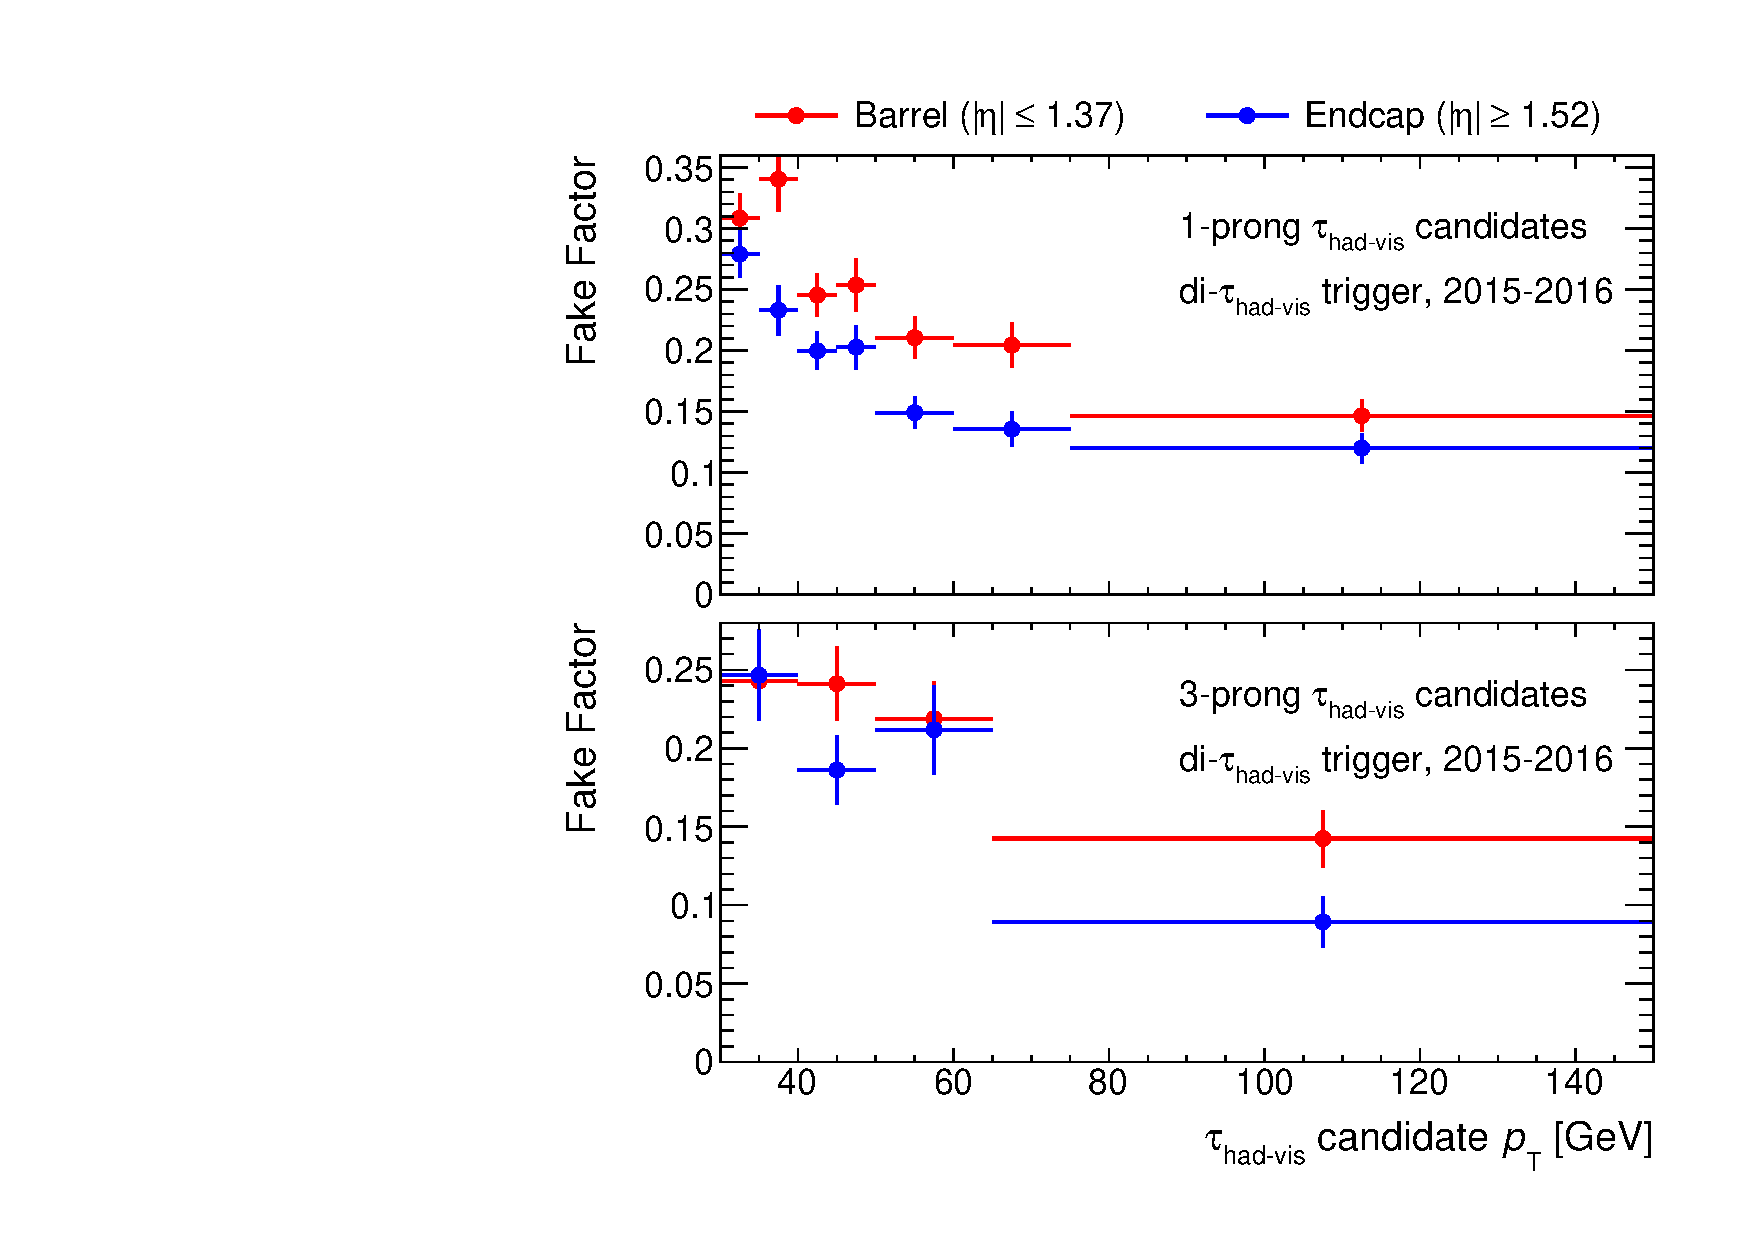
\includegraphics[width=\textwidth]{fakefactors/fake_factors_dtt_1516}
    \subcaption{DTT fake factors measured using 2015-2016 data}
  \end{subfigure}
  \begin{subfigure}{0.49\textwidth}
    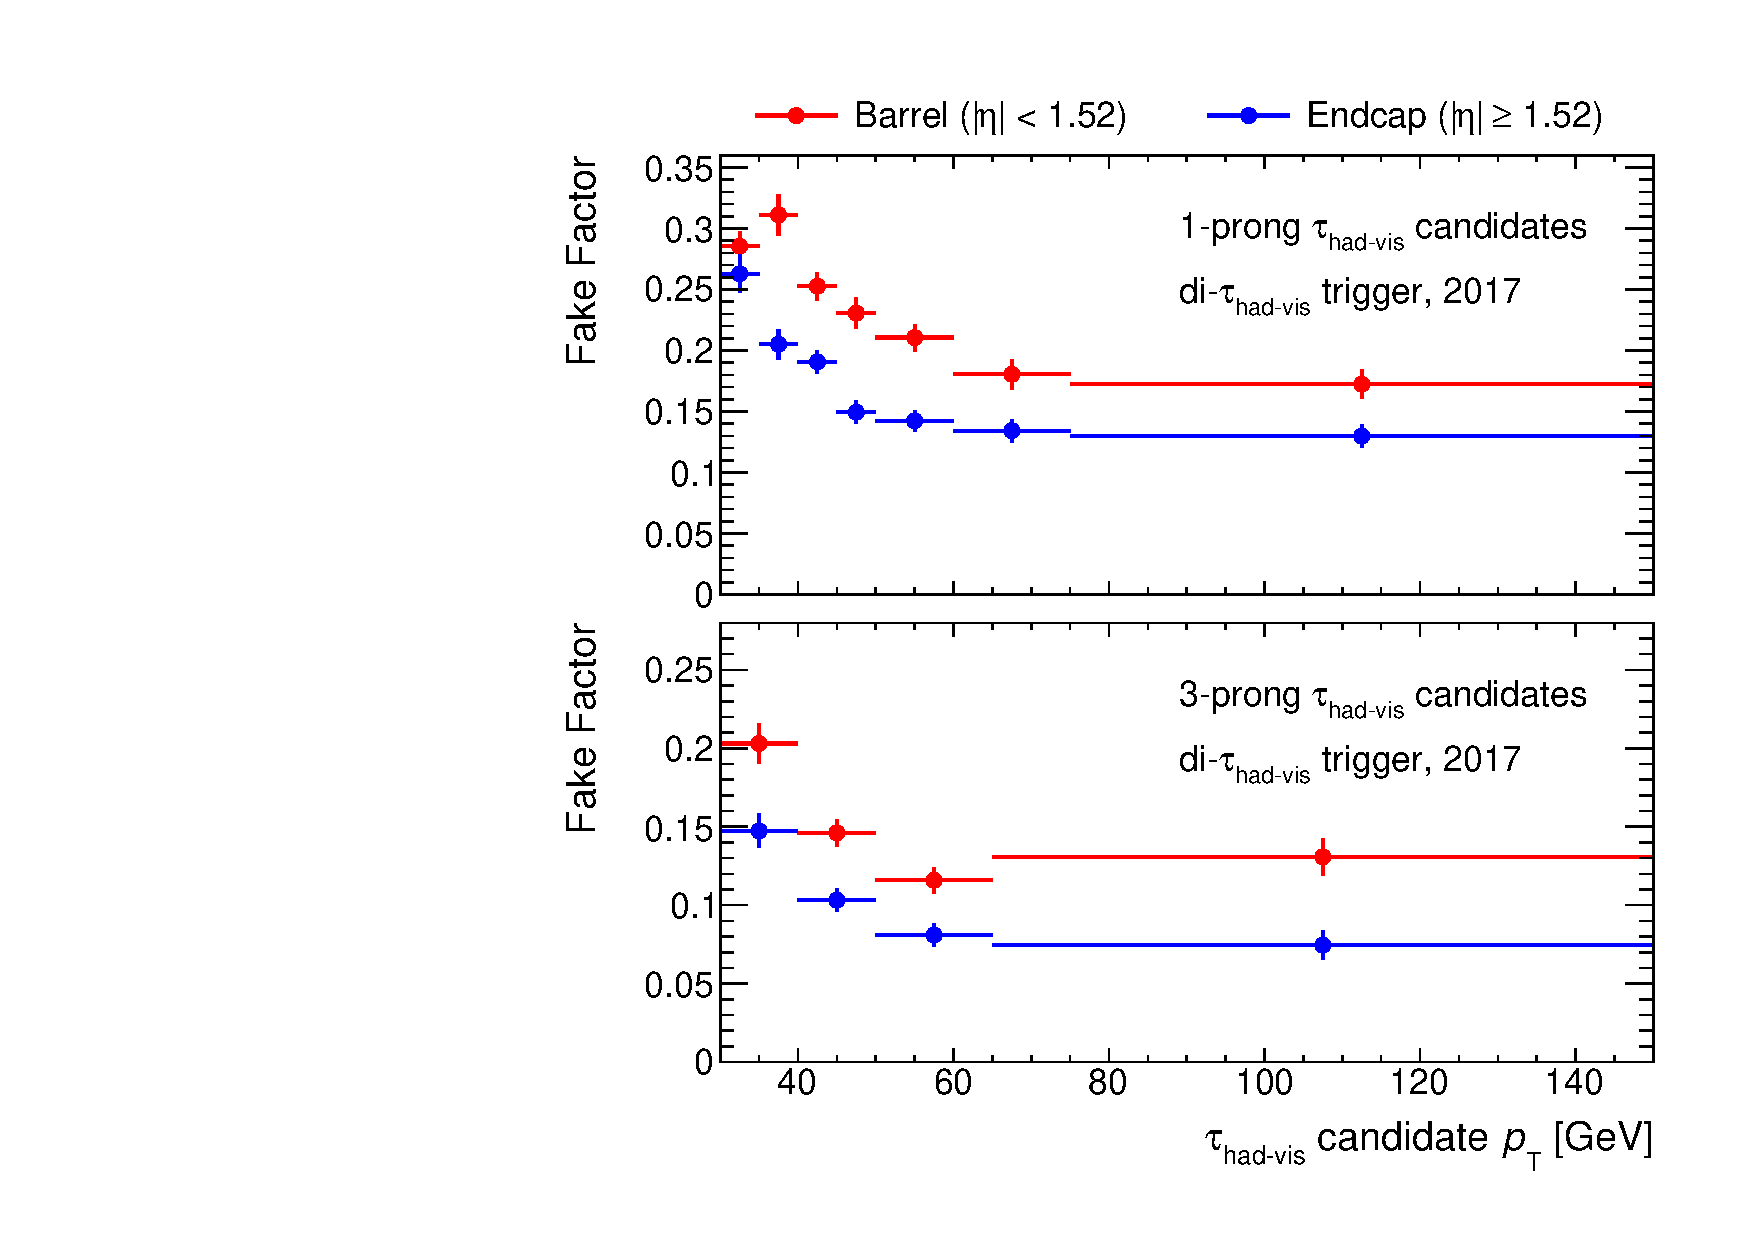
\includegraphics[width=\textwidth]{fakefactors/fake_factors_dtt_17}
    \subcaption{DTT fake factors measured using 2017 data}
  \end{subfigure}

  \begin{subfigure}{0.49\textwidth}
    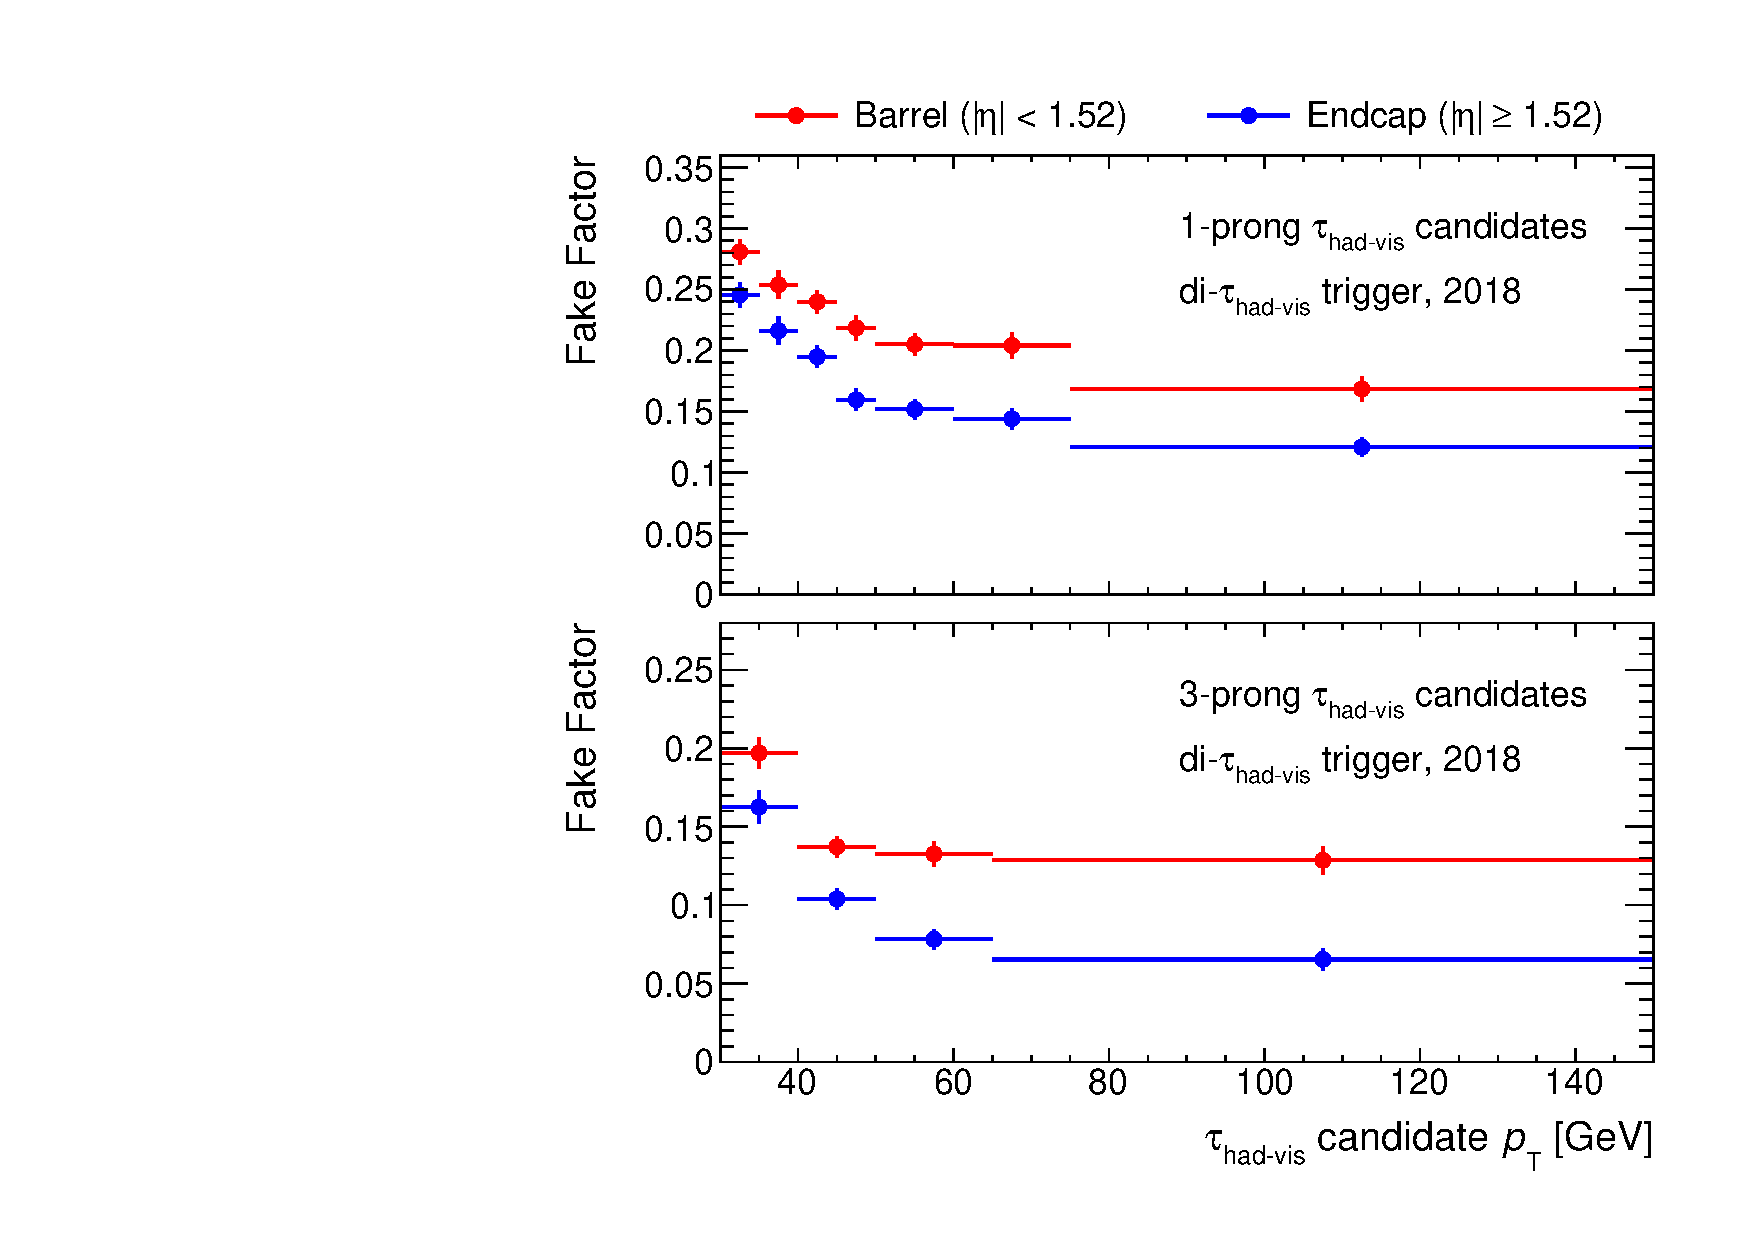
\includegraphics[width=\textwidth]{fakefactors/fake_factors_dtt_18}
    \subcaption{DTT fake factors measured using 2018 data}
  \end{subfigure}

  \caption{Combined Fake Factors DTT. The last bin is inclusive in all
    \pT larger than \SI{150}{\GeV}.}
  \label{fig:mjfakes_fake_factors}
\end{figure}



% - STT fake factors
Here it makes a difference whether the leading or the subleading tau
is an anti-\tauhadvis since this entails a particular \pT distribtion
(and the FFs are not binned in \pT).


% Additional info that would be interesting:
% - Subtraction

\begin{figure}[htbp]
  \centering

  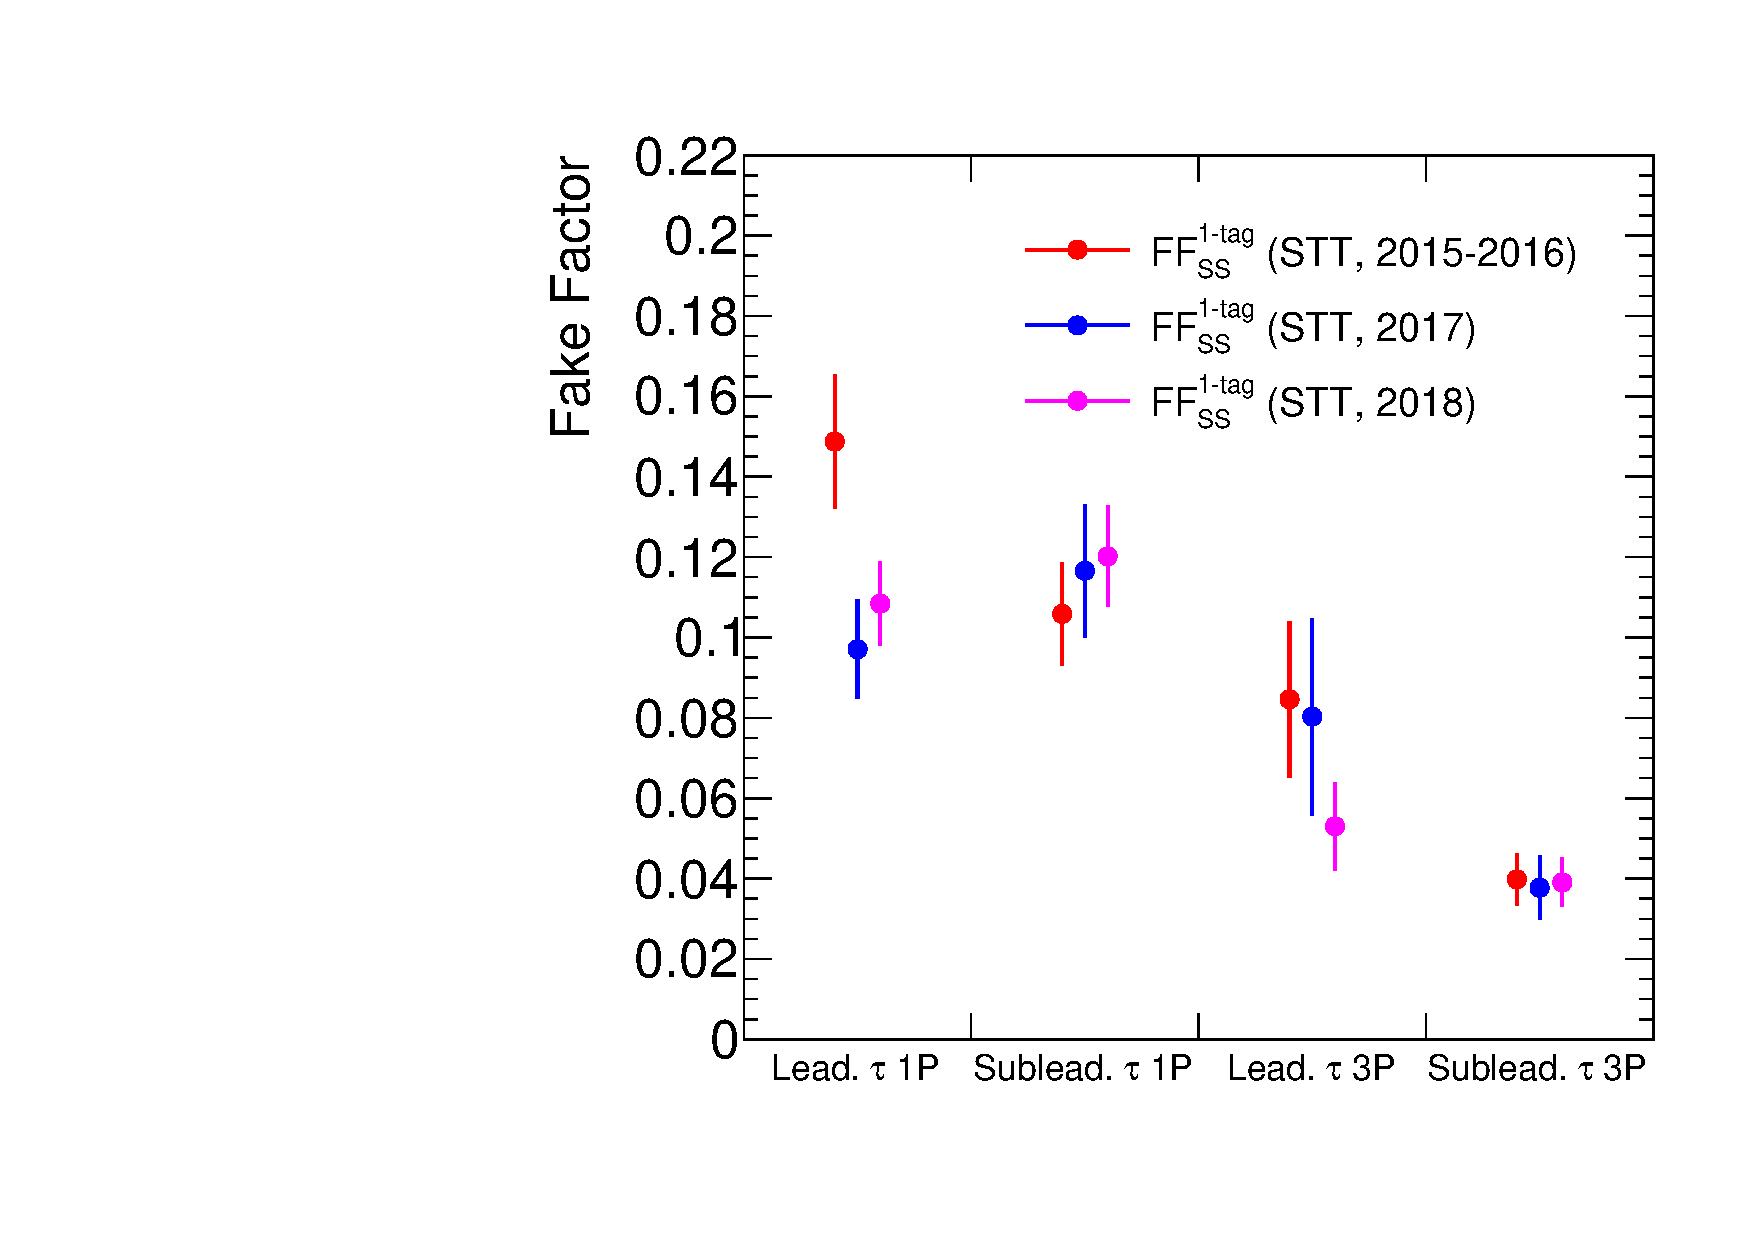
\includegraphics[width=0.45\textwidth]{fakefactors/fake_factors_stt}

  \todo[inline]{Largest deviation for leading 1-prong tau possibly due
    to looser pT threshold.}

  \caption{STT fake factors}
  \label{fig:mjfakes_stt_ffs}
\end{figure}


\begin{figure}[htbp]
  \centering

  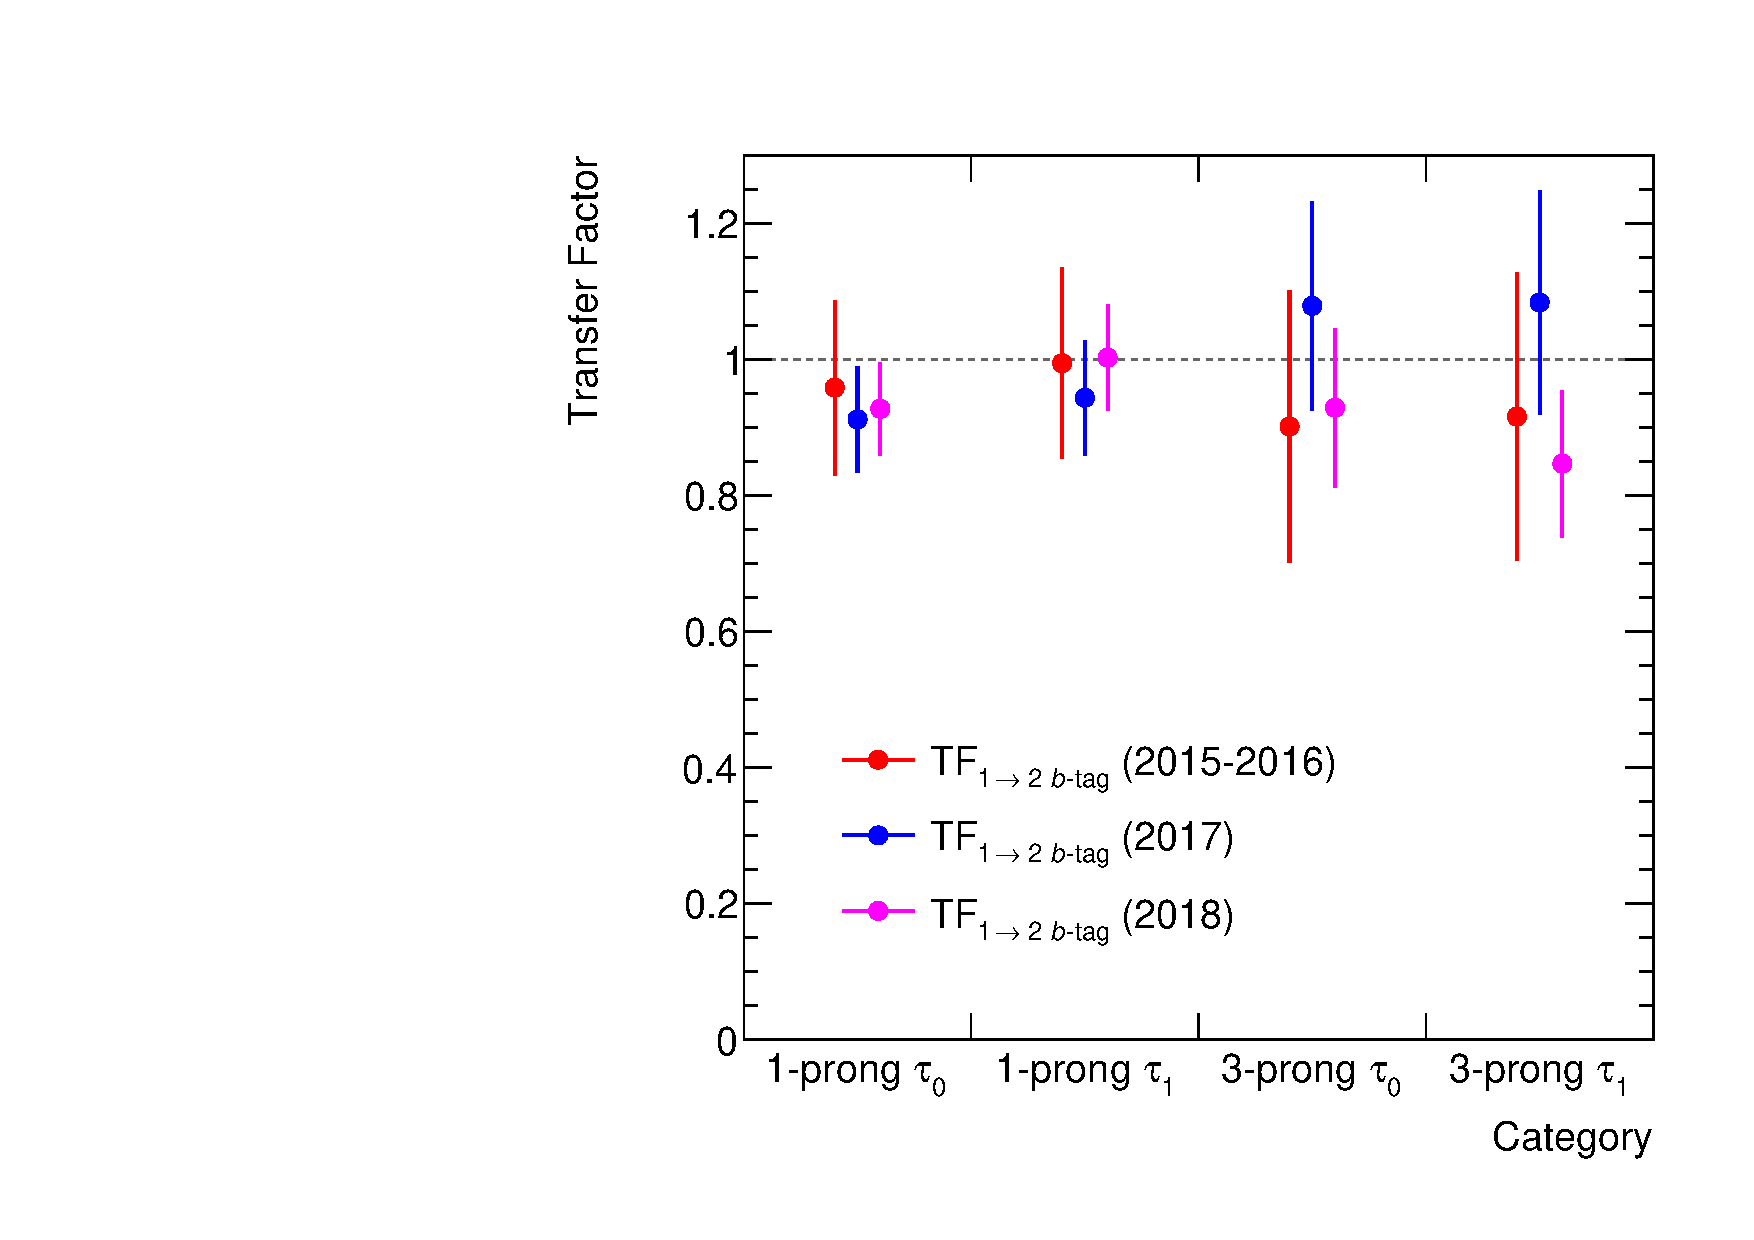
\includegraphics[width=0.45\textwidth]{fakefactors/transfer_factors}

  \caption{Transfer Factors}
  \label{fig:mjfakes_transfer_factor}
\end{figure}


\subsubsection{Estimation of multi-jet backgrounds in the signal region}

% - Transfer factor calculation
% - Subtraction in Anti-ID region

\subsubsection{Systematic Uncertainties}

% - Uncertainties


% The fake factors are not expected to depend strongly
% on the applied \btag requirement

% Dominant subtraction is ttbar, execpt for 1-tag OS ID where it is
% Ztautau.

% Signal contamination / other background contamination

% Yield table / plots of regions

% Checked in 1-tag OS. Does agreement in 1-tag OS confirm that charge
% and ID are independent? Closure, yes

\todo[inline]{Old stuff below:}

The fake factor (FF) measures the ratio of events with fake \tauhadvis in ID and
Anti-ID region:
\begin{align*}
  \FF = \frac{N\left( \text{fake} \, \tauhadvis, \text{ID} \right)}{N\left( \text{fake} \, \tauhadvis, \text{Anti-ID} \right)}
\end{align*}
The probability of a jet faking a \tauhadvis depends strongly on \tauhadvis \pT
and decay mode. Therefore, the fake factor is frequently parametrised in these
quantities. It is also affected by the \tauhadvis identification already applied
in the high-level \tauhadvis-triggers which also needs to be taken into account.

The fake factors are measured in the fake enriched SS-region by subtracting
non-fake-\tauhadvis background using their estimates from simulation:
\begin{align*}
  \FF_\text{SS} = \frac{N(\text{SS}, \text{ID}) - N_\text{non-fake}(\text{SS}, \text{ID})}{N(\text{SS}, \text{Anti-ID}) - N_\text{non-fake}(\text{SS}, \text{Anti-ID})}
\end{align*}
where $N$ is the total yield and $N_\text{non-fake}$ the yield of
non-fake-\tauhadvis backgrounds in the corresponding region.

To obtain the fake \tauhadvis estimate in the OS ID-region, the assumption is
made that the fake factors are independent of the reconstructed charge of the
fake \tauhadvis candidates. Therefore, the SS fake factors $\FF_\text{SS}$ are
applied to events in the OS Anti-ID region after subtracting any
non-fake-\tauhadvis contributions.
\begin{align*}
  N(\text{fake}, \text{OS ID}) = \FF_\text{SS} \times \left[ N(\text{OS}, \text{Anti-ID}) - N_\text{non-fake}(\text{OS}, \text{Anti-ID}) \right]
\end{align*}
Systematic uncertainties are assigned to
cover possible difference betwen OS and SS fake factors, varying the
subtraction in the OS Anti-ID region. Moreover, the fake factors are
independently varied by their statistical uncertainty.

Due to the limited acceptance of fake \tauhadvis in the 2 \btag region, the 1
\btag region is used to calculate the fake factors instead. The 1 \btag fake
factors are applied to the 2 \btag OS Anti-ID region and an additional 1 to 2
\btag transfer factor is applied.

The binning of the fake factors is dependent on the trigger that selected the
event. For STT events the fake factor is binned in whether the anti-\tauhadvis
is leading or subleading in \pT, and the decay mode of the \tauhadvis
($N_\text{track}$). Due to low statistics in the STT category the fake factors
are inclusive in \tauhadvis \pT. The \tauhadvis identification at the HLT is
only applied to one of the two \tauhadvis candidates affecting the probability
of jets faking \tauhadvis, motivating the binning in whether the leading /
subleading \tauhadvis fails the identification.

For DTT events, HLT \tauhadvis identification is applied to both \tauhadvis
candidates. Therefore, the fake factors do not need to distinguish between cases
where the leading and subleading \tauhadvis fails the loose identification. The
fake factors for DTT events are parametrised in the \pT and decay mode of the
the \tauhadvis candidate failing the identification requirement.

Moreover, all fake factors are binned by data-taking period (${\text{2015-2016},
  \text{2017}, \text{2018}}$) which takes into account the different triggers
being used to select events used for the analysis.

\todo[inline]{Could we use nOS to enhance statistics? Maybe flip the FF method
  so that we use events in SS ID to build the template instead of OS Anti-ID.}

\todo[inline]{Can we make the STT FF depend on the trigger-match instead of
  the leading / subleading binning?}









%%% Local Variables:
%%% mode: latex
%%% TeX-master: "../../phd_thesis"
%%% End:
